\documentclass{standalone}
\usepackage{tikz}
\usetikzlibrary{patterns, positioning}

\begin{document}
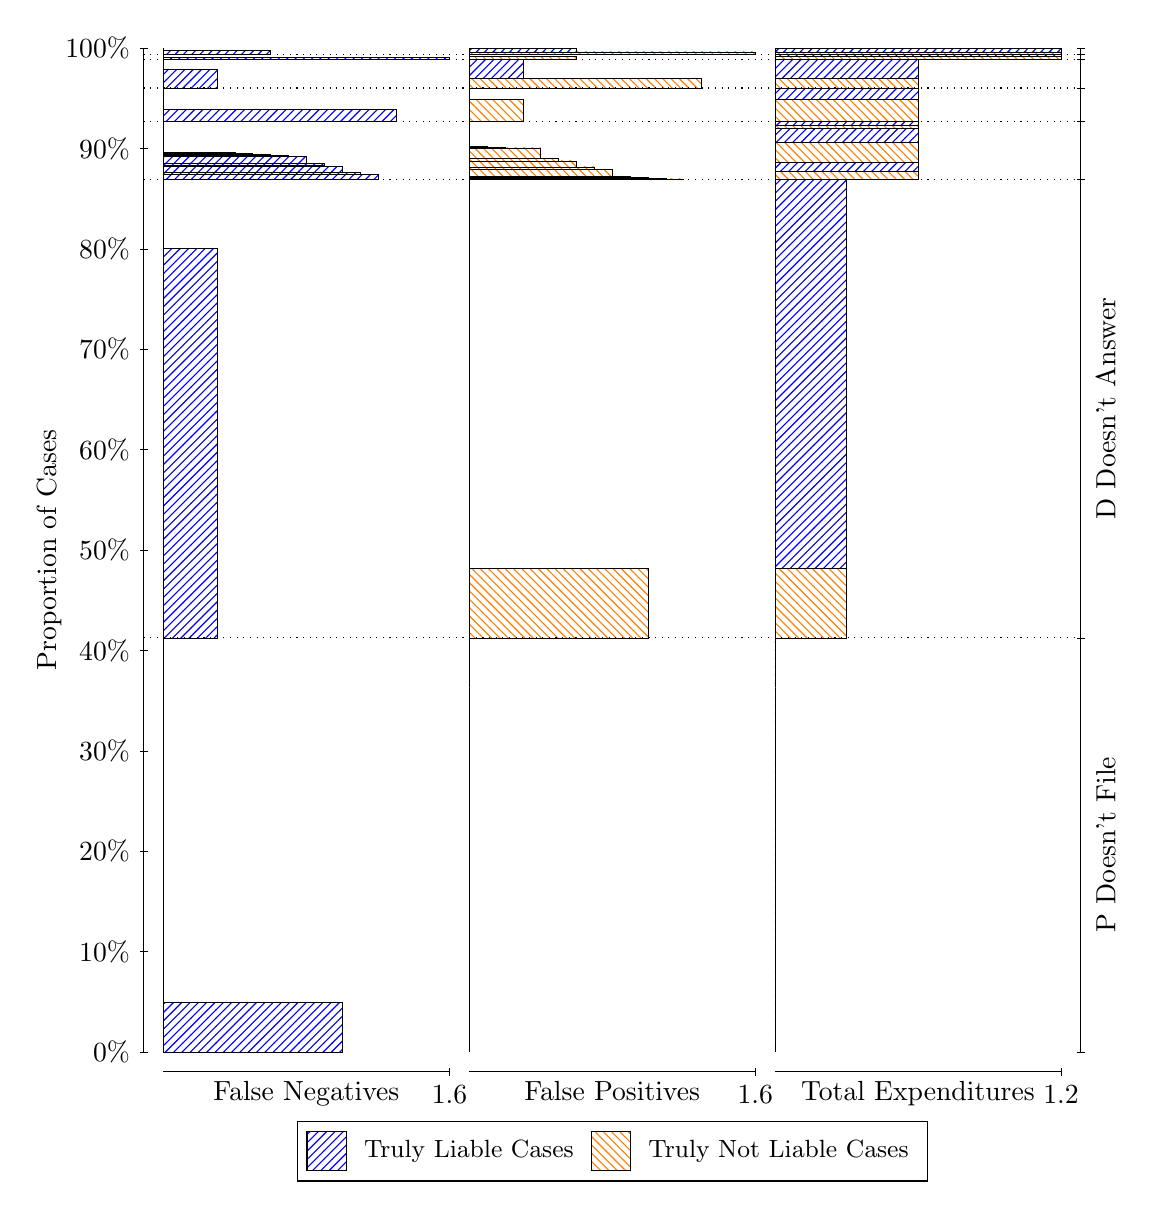
\begin{tikzpicture}
\draw[black, very thin] (1.5,1.75) -- (1.5,14.5);
\node[rotate=90, anchor=center] at (0.3, 8.125) {Proportion of Cases};
\draw[black, very thin] (1.45,1.75) -- (1.55,1.75);
\node[anchor=east] at (1.45, 1.75) {0\%};
\draw[black, very thin] (1.45,3.025) -- (1.55,3.025);
\node[anchor=east] at (1.45, 3.025) {10\%};
\draw[black, very thin] (1.45,4.3) -- (1.55,4.3);
\node[anchor=east] at (1.45, 4.3) {20\%};
\draw[black, very thin] (1.45,5.575) -- (1.55,5.575);
\node[anchor=east] at (1.45, 5.575) {30\%};
\draw[black, very thin] (1.45,6.85) -- (1.55,6.85);
\node[anchor=east] at (1.45, 6.85) {40\%};
\draw[black, very thin] (1.45,8.125) -- (1.55,8.125);
\node[anchor=east] at (1.45, 8.125) {50\%};
\draw[black, very thin] (1.45,9.4) -- (1.55,9.4);
\node[anchor=east] at (1.45, 9.4) {60\%};
\draw[black, very thin] (1.45,10.675) -- (1.55,10.675);
\node[anchor=east] at (1.45, 10.675) {70\%};
\draw[black, very thin] (1.45,11.95) -- (1.55,11.95);
\node[anchor=east] at (1.45, 11.95) {80\%};
\draw[black, very thin] (1.45,13.225) -- (1.55,13.225);
\node[anchor=east] at (1.45, 13.225) {90\%};
\draw[black, very thin] (1.45,14.5) -- (1.55,14.5);
\node[anchor=east] at (1.45, 14.5) {100\%};

\draw[black, very thin] (13.4,1.75) -- (13.4,14.5);
\draw[black, very thin] (13.35,1.75) -- (13.45,1.75);
\node[anchor=west] at (13.35, 1.75) {};
\draw[black, very thin] (13.35,7.01) -- (13.45,7.01);
\node[anchor=west] at (13.35, 7.01) {};
\draw[black, very thin] (13.35,12.833) -- (13.45,12.833);
\node[anchor=west] at (13.35, 12.833) {};
\draw[black, very thin] (13.35,13.569) -- (13.45,13.569);
\node[anchor=west] at (13.35, 13.569) {};
\draw[black, very thin] (13.35,13.992) -- (13.45,13.992);
\node[anchor=west] at (13.35, 13.992) {};
\draw[black, very thin] (13.35,14.354) -- (13.45,14.354);
\node[anchor=west] at (13.35, 14.354) {};
\draw[black, very thin] (13.35,14.422) -- (13.45,14.422);
\node[anchor=west] at (13.35, 14.422) {};
\draw[black, very thin] (13.35,14.5) -- (13.45,14.5);
\node[anchor=west] at (13.35, 14.5) {};

\draw[black, very thin, pattern color=blue, pattern=north east lines] (1.75,1.75) rectangle (4.0208,2.3828);
\draw[black, very thin, pattern color=orange, pattern=north west lines] (1.75,2.3828) rectangle (1.75,7.01);
\draw[black, very thin, pattern color=blue, pattern=north east lines] (1.75,7.01) rectangle (2.4312,11.954);
\draw[black, very thin, pattern color=orange, pattern=north west lines] (1.75,11.954) rectangle (1.75,12.833);
\draw[black, very thin, pattern color=blue, pattern=north east lines] (1.75,12.833) rectangle (4.475,12.9);
\draw[black, very thin, pattern color=blue, pattern=north east lines] (1.75,12.9) rectangle (4.2479,12.924);
\draw[black, very thin, pattern color=blue, pattern=north east lines] (1.75,12.924) rectangle (4.0208,13);
\draw[black, very thin, pattern color=blue, pattern=north east lines] (1.75,13) rectangle (3.7937,13.01);
\draw[black, very thin, pattern color=blue, pattern=north east lines] (1.75,13.01) rectangle (3.7937,13.034);
\draw[black, very thin, pattern color=blue, pattern=north east lines] (1.75,13.034) rectangle (3.5667,13.122);
\draw[black, very thin, pattern color=blue, pattern=north east lines] (1.75,13.122) rectangle (3.3396,13.136);
\draw[black, very thin, pattern color=blue, pattern=north east lines] (1.75,13.136) rectangle (3.1125,13.153);
\draw[black, very thin, pattern color=blue, pattern=north east lines] (1.75,13.153) rectangle (2.8854,13.159);
\draw[black, very thin, pattern color=blue, pattern=north east lines] (1.75,13.159) rectangle (2.6583,13.171);
\draw[black, very thin, pattern color=orange, pattern=north west lines] (1.75,13.171) rectangle (1.75,13.569);
\draw[black, very thin, pattern color=blue, pattern=north east lines] (1.75,13.569) rectangle (4.7021,13.717);
\draw[black, very thin, pattern color=orange, pattern=north west lines] (1.75,13.717) rectangle (1.75,13.992);
\draw[black, very thin, pattern color=blue, pattern=north east lines] (1.75,13.992) rectangle (2.4312,14.228);
\draw[black, very thin, pattern color=orange, pattern=north west lines] (1.75,14.228) rectangle (1.75,14.354);
\draw[black, very thin, pattern color=blue, pattern=north east lines] (1.75,14.354) rectangle (5.3833,14.381);
\draw[black, very thin, pattern color=orange, pattern=north west lines] (1.75,14.381) rectangle (1.75,14.422);
\draw[black, very thin, pattern color=blue, pattern=north east lines] (1.75,14.422) rectangle (3.1125,14.472);
\draw[black, very thin, pattern color=orange, pattern=north west lines] (1.75,14.472) rectangle (1.75,14.5);
\draw[black, very thin, pattern color=orange, pattern=north west lines] (5.6333,1.75) rectangle (5.6333,6.3773);
\draw[black, very thin, pattern color=blue, pattern=north east lines] (5.6333,6.3773) rectangle (5.6333,7.01);
\draw[black, very thin, pattern color=orange, pattern=north west lines] (5.6333,7.01) rectangle (7.9042,7.8891);
\draw[black, very thin, pattern color=blue, pattern=north east lines] (5.6333,7.8891) rectangle (5.6333,12.833);
\draw[black, very thin, pattern color=orange, pattern=north west lines] (5.6333,12.833) rectangle (8.3583,12.838);
\draw[black, very thin, pattern color=orange, pattern=north west lines] (5.6333,12.838) rectangle (8.1313,12.842);
\draw[black, very thin, pattern color=orange, pattern=north west lines] (5.6333,12.842) rectangle (7.9042,12.856);
\draw[black, very thin, pattern color=orange, pattern=north west lines] (5.6333,12.856) rectangle (7.6771,12.869);
\draw[black, very thin, pattern color=orange, pattern=north west lines] (5.6333,12.869) rectangle (7.45,12.957);
\draw[black, very thin, pattern color=orange, pattern=north west lines] (5.6333,12.957) rectangle (7.2229,12.99);
\draw[black, very thin, pattern color=orange, pattern=north west lines] (5.6333,12.99) rectangle (6.9958,13.068);
\draw[black, very thin, pattern color=orange, pattern=north west lines] (5.6333,13.068) rectangle (6.7687,13.097);
\draw[black, very thin, pattern color=orange, pattern=north west lines] (5.6333,13.097) rectangle (6.5417,13.231);
\draw[black, very thin, pattern color=blue, pattern=north east lines] (5.6333,13.231) rectangle (6.0875,13.243);
\draw[black, very thin, pattern color=blue, pattern=north east lines] (5.6333,13.243) rectangle (5.8604,13.25);
\draw[black, very thin, pattern color=blue, pattern=north east lines] (5.6333,13.25) rectangle (5.6333,13.569);
\draw[black, very thin, pattern color=orange, pattern=north west lines] (5.6333,13.569) rectangle (6.3146,13.844);
\draw[black, very thin, pattern color=blue, pattern=north east lines] (5.6333,13.844) rectangle (5.6333,13.992);
\draw[black, very thin, pattern color=orange, pattern=north west lines] (5.6333,13.992) rectangle (8.5854,14.118);
\draw[black, very thin, pattern color=blue, pattern=north east lines] (5.6333,14.118) rectangle (6.3146,14.354);
\draw[black, very thin, pattern color=orange, pattern=north west lines] (5.6333,14.354) rectangle (6.9958,14.395);
\draw[black, very thin, pattern color=blue, pattern=north east lines] (5.6333,14.395) rectangle (5.6333,14.422);
\draw[black, very thin, pattern color=orange, pattern=north west lines] (5.6333,14.422) rectangle (9.2667,14.45);
\draw[black, very thin, pattern color=blue, pattern=north east lines] (5.6333,14.45) rectangle (6.9958,14.5);
\draw[black, very thin, pattern color=orange, pattern=north west lines] (9.5167,1.75) rectangle (9.5167,6.3773);
\draw[black, very thin, pattern color=blue, pattern=north east lines] (9.5167,6.3773) rectangle (9.5167,7.01);
\draw[black, very thin, pattern color=orange, pattern=north west lines] (9.5167,7.01) rectangle (10.425,7.8891);
\draw[black, very thin, pattern color=blue, pattern=north east lines] (9.5167,7.8891) rectangle (10.425,12.833);
\draw[black, very thin, pattern color=orange, pattern=north west lines] (9.5167,12.833) rectangle (11.333,12.938);
\draw[black, very thin, pattern color=blue, pattern=north east lines] (9.5167,12.938) rectangle (11.333,13.05);
\draw[black, very thin, pattern color=orange, pattern=north west lines] (9.5167,13.05) rectangle (11.333,13.3);
\draw[black, very thin, pattern color=blue, pattern=north east lines] (9.5167,13.3) rectangle (11.333,13.477);
\draw[black, very thin, pattern color=orange, pattern=north west lines] (9.5167,13.477) rectangle (11.333,13.519);
\draw[black, very thin, pattern color=blue, pattern=north east lines] (9.5167,13.519) rectangle (11.333,13.569);
\draw[black, very thin, pattern color=orange, pattern=north west lines] (9.5167,13.569) rectangle (11.333,13.844);
\draw[black, very thin, pattern color=blue, pattern=north east lines] (9.5167,13.844) rectangle (11.333,13.992);
\draw[black, very thin, pattern color=orange, pattern=north west lines] (9.5167,13.992) rectangle (11.333,14.118);
\draw[black, very thin, pattern color=blue, pattern=north east lines] (9.5167,14.118) rectangle (11.333,14.354);
\draw[black, very thin, pattern color=orange, pattern=north west lines] (9.5167,14.354) rectangle (13.15,14.395);
\draw[black, very thin, pattern color=blue, pattern=north east lines] (9.5167,14.395) rectangle (13.15,14.422);
\draw[black, very thin, pattern color=orange, pattern=north west lines] (9.5167,14.422) rectangle (13.15,14.45);
\draw[black, very thin, pattern color=blue, pattern=north east lines] (9.5167,14.45) rectangle (13.15,14.5);
\draw[black, dotted] (1.5,7.01) -- (13.4,7.01);
\draw[black, dotted] (1.5,12.833) -- (13.4,12.833);
\draw[black, dotted] (1.5,13.569) -- (13.4,13.569);
\draw[black, dotted] (1.5,13.992) -- (13.4,13.992);
\draw[black, dotted] (1.5,14.354) -- (13.4,14.354);
\draw[black, dotted] (1.5,14.422) -- (13.4,14.422);
\draw[black, very thin] (1.75,1.5) -- (5.3833,1.5);
\node[anchor=north] at (3.5667, 1.5) {False Negatives};
\draw[black, very thin] (5.3833,1.45) -- (5.3833,1.55);
\node[anchor=north] at (5.3833, 1.45) {1.6};

\draw[black, very thin] (5.6333,1.5) -- (9.2667,1.5);
\node[anchor=north] at (7.45, 1.5) {False Positives};
\draw[black, very thin] (9.2667,1.45) -- (9.2667,1.55);
\node[anchor=north] at (9.2667, 1.45) {1.6};

\draw[black, very thin] (9.5167,1.5) -- (13.15,1.5);
\node[anchor=north] at (11.333, 1.5) {Total Expenditures};
\draw[black, very thin] (13.15,1.45) -- (13.15,1.55);
\node[anchor=north] at (13.15, 1.45) {1.2};

\node[black, centered, rotate=90] at (13.72, 4.38) {P Doesn't File};
\node[black, centered, rotate=90] at (13.72, 9.9216) {D Doesn't Answer};






\draw (7.449999999999999,1.5) node[draw=none] (baseCoordinate) {};
\begin{scope}[align=center]
        \matrix[scale=0.5, draw=black, below=0.5cm of baseCoordinate, nodes={draw}, column sep=0.1cm]{
            \node[rectangle, draw, minimum width=0.5cm, minimum height=0.5cm, pattern=north east lines, pattern color=blue] {}; &
            \node[draw=none, font=\small] (B) {Truly Liable Cases}; &
            \node[rectangle, draw, minimum width=0.5cm, minimum height=0.5cm, pattern=north west lines, pattern color=orange] {}; &
            \node[draw=none, font=\small] (B) {Truly Not Liable Cases}; \\
            };
\end{scope}

\end{tikzpicture}
\end{document}